\chapter{Experimental Results}

\section{Data on models used}

\section{Different resolutions, Bunny model}
\begin{tabularx}{\textwidth}{|r|X|} \hline
Method & ICP. Select all points, closest point criterion, equal weights, no rejection, point-to-point error metric. \\ \hline
Model & Stanford Bunny model. \\ \hline
Fixed & 50\% of model points, randomly chosen. \\ \hline
Loose & Starting from the other 50\%, randomly downsampled by given amount. $60$ steps. \\ \hline
Displacement & See captions on the figures. \\ \hline
Y Axis & True error, after $40$ iterations. \\\hline
X Axis & Number of points in Loose divided by number of points in Fixed. \\ \hline
\end{tabularx}


\subsection{Final true error v. downsampling level} \label{sec:bunny_hilo}

\begin{figure}[H]
\centering
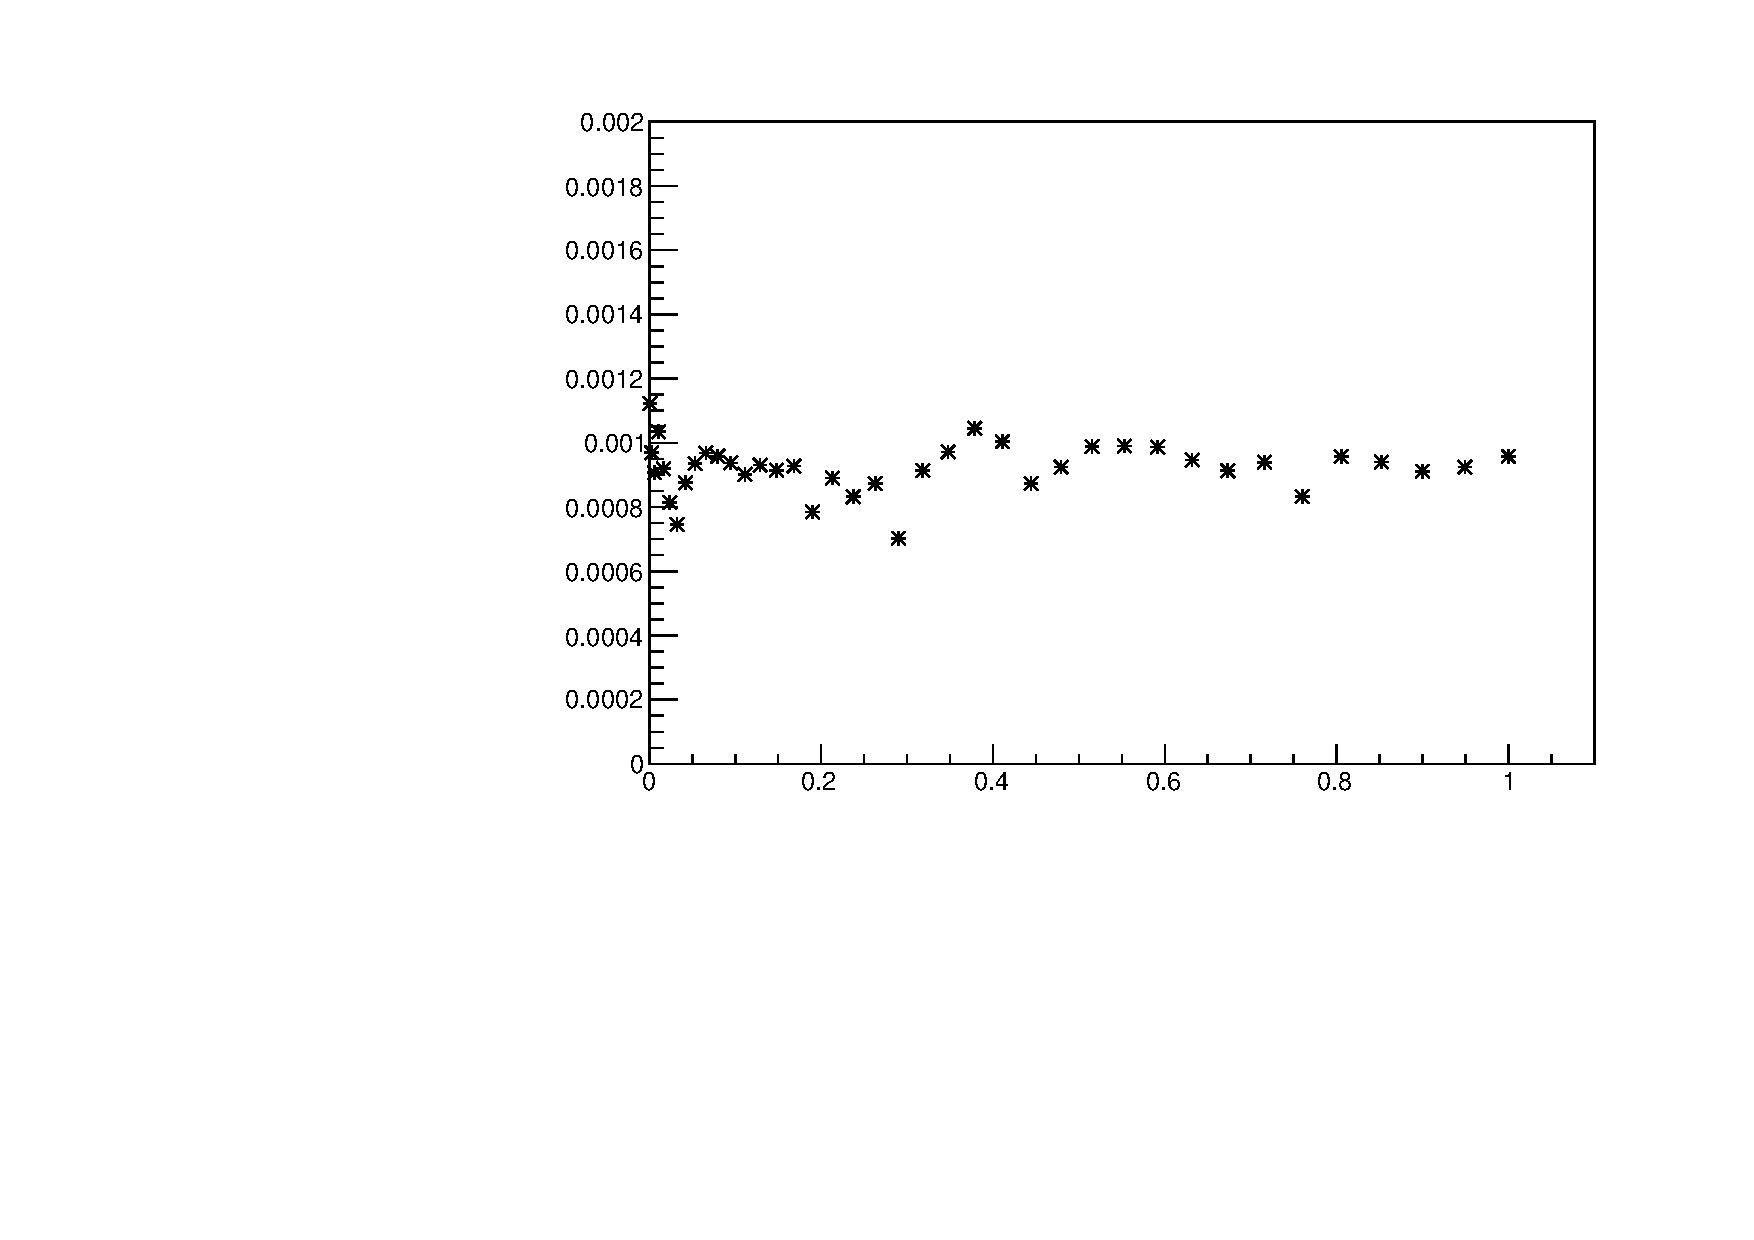
\includegraphics[width=.7\textwidth]{fig/bunny_globmin.pdf}
\caption{no displacement}
\label{fig:bunny_globmin}
\end{figure}
\begin{figure}[H]
\centering
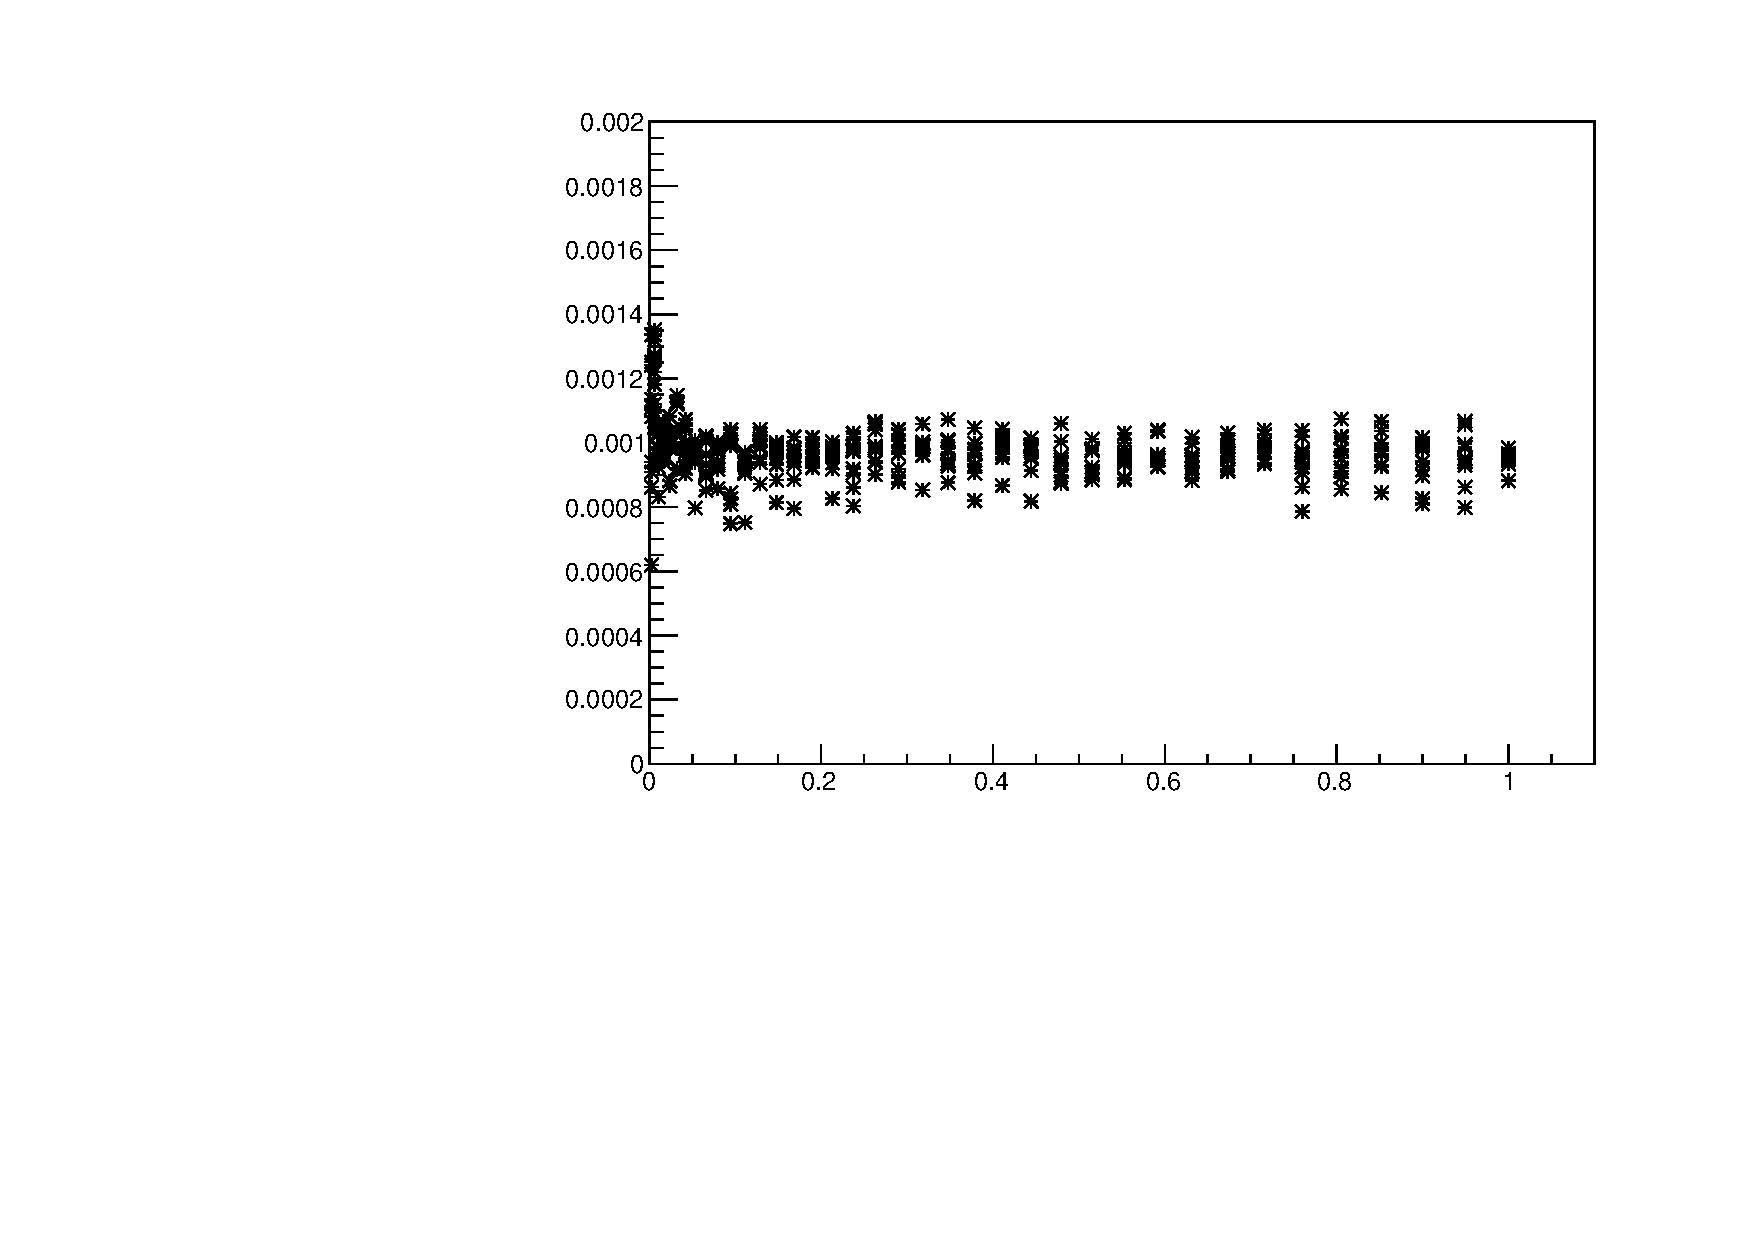
\includegraphics[width=.7\textwidth]{fig/bunny_globsmall.pdf}
\caption{random translation of $0.01$ and rotation of $3 \si{\degree}$, chosen $10$ times}
\label{fig:bunny_globsmall}
\end{figure}
\begin{figure}[H]
\centering
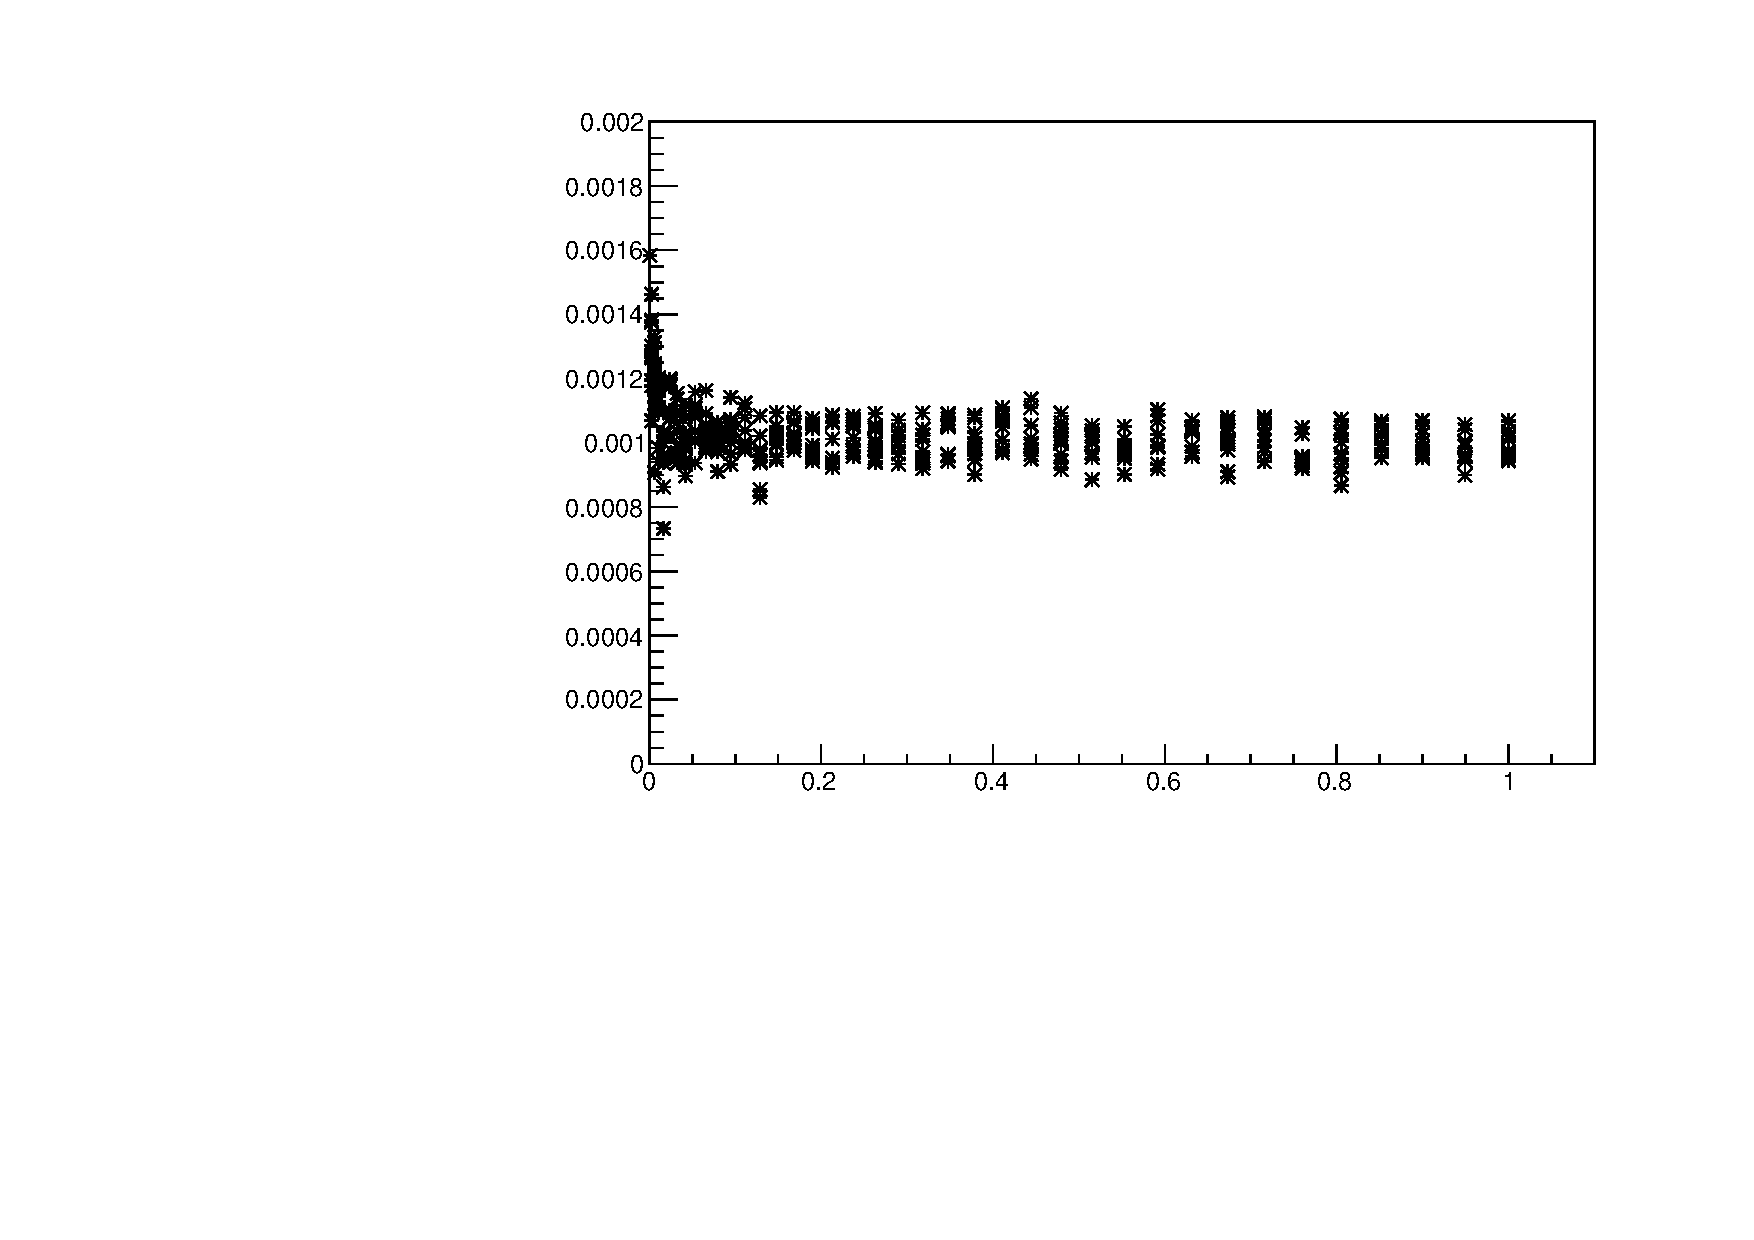
\includegraphics[width=.7\textwidth]{fig/bunny_globmed.pdf}
\caption{random translation of $0.01$ and rotation of $15 \si{\degree}$, chosen $10$ times}
\label{fig:bunny_globmed}
\end{figure}

\begin{figure}[H]
\centering
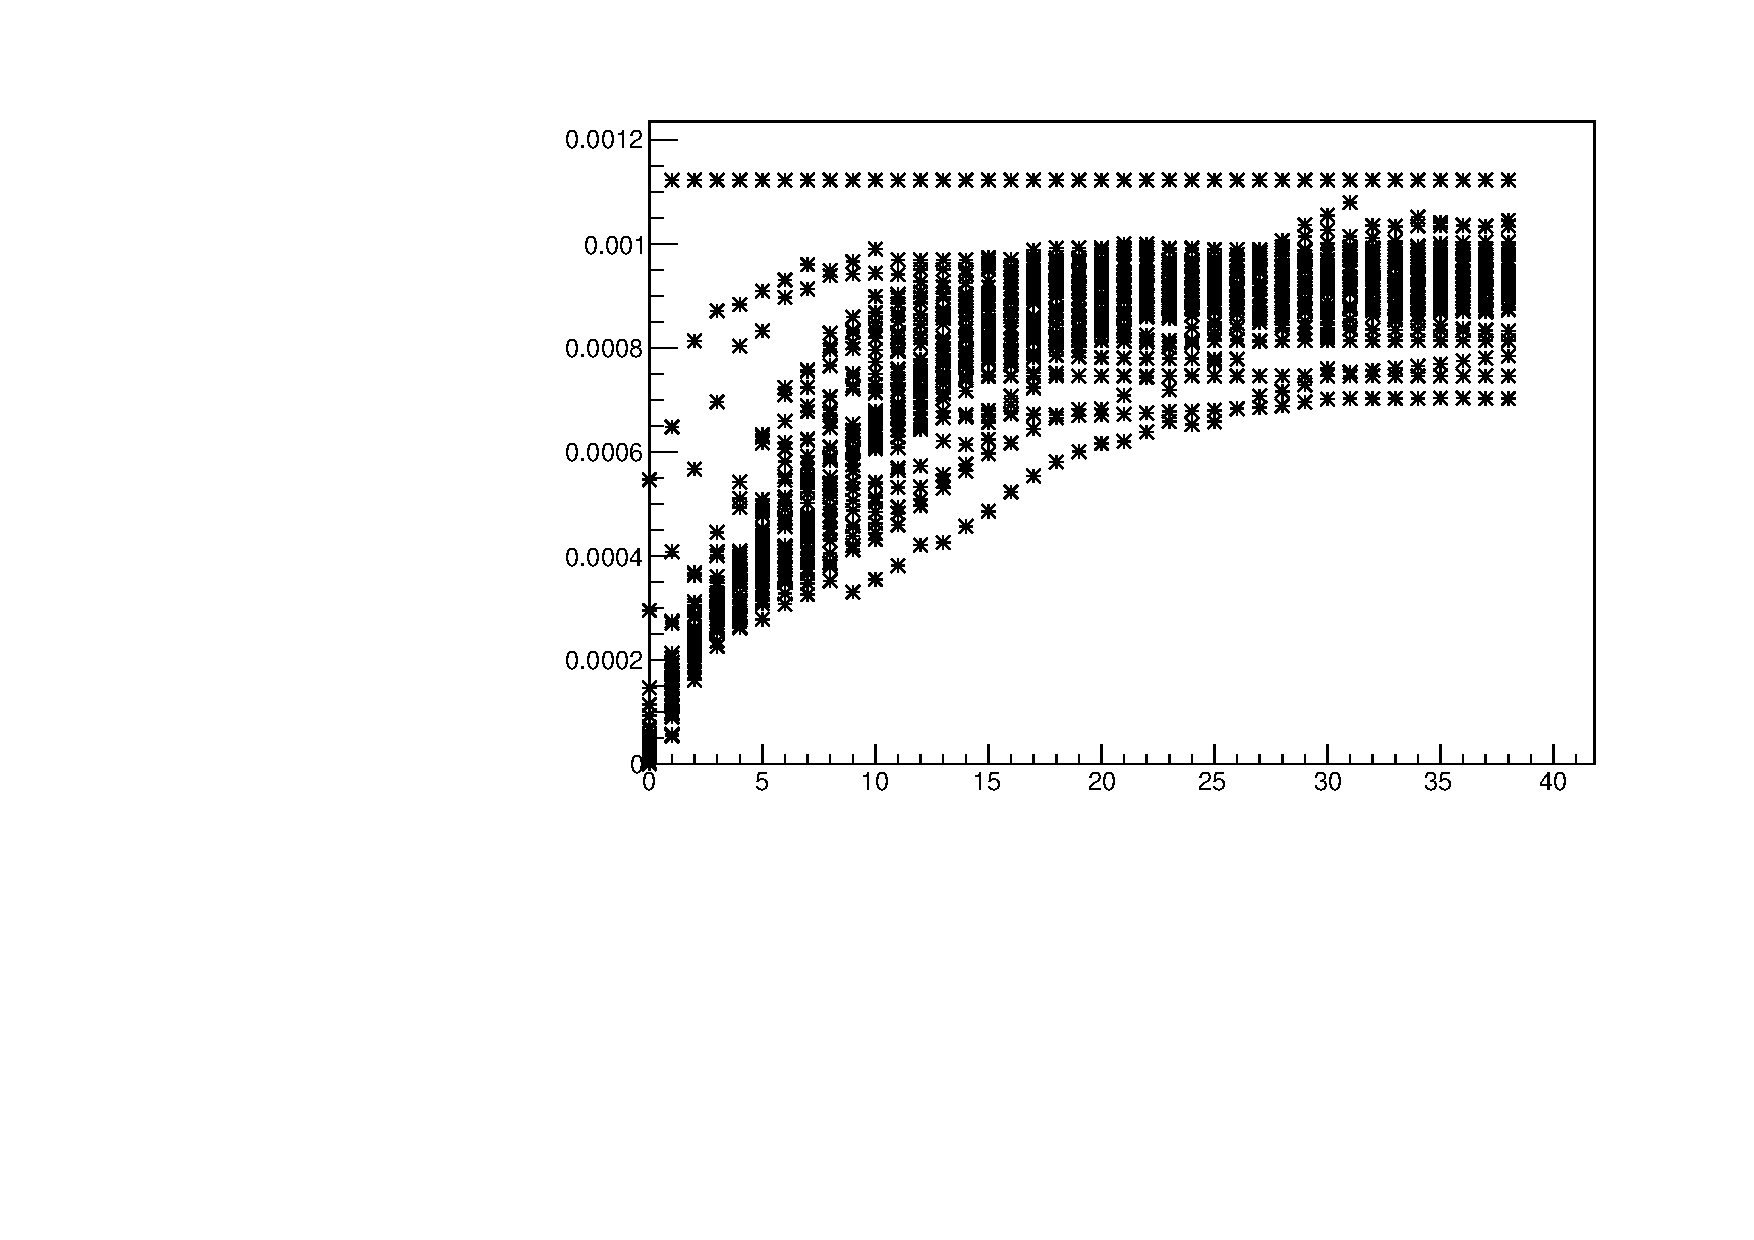
\includegraphics[width=.7\textwidth]{fig/bunny_globmin_ev.pdf}
\caption{Evolutions of true error for experiment \ref{ref:bunny_hilo_a}}
\label{ref:bunny_hilo_ev}
\end{figure}
